%!TEX TS-program = xelatex
%!TEX encoding = UTF-8 Unicode
%!TEX root = 2022-GS-ARTICLE.tex
%----------------------------------------------------------------- LANGUAGES ---
\newcommand{\mylanguages}{italian} % in reverse order
%---------------------------------------------------------- TITLE & SUBTITLE ---
\newcommand{\mytitle}{Totalità sonora: il corpo dell'orchestra}
\newcommand{\mysubtitle}{Per ascoltare l'organismo sonoro orchestrale nel suo complesso e nei singoli dettagli}
%----------------------------------------------------------------- AUTHOR(s) ---
\newcommand{\authorone}{Giancarlo Bottalico}
\newcommand{\institutione}{Conservatorio di musica "N. Piccinni", Bari}
\newcommand{\emailone}{giancarlobottalico@gmail.com}
%-------------------------------------------------------------------------------
% \newcommand{\authortwo}{Wikio Orgopedio}
% \newcommand{\institutiontwo}{Conservatorio S. Cecilia di Roma}
% \newcommand{\emailtwo}{wikio @ orgopedio.com} % duplicate these 3 lines if more
%-------------------------------------------------------------- STYLE GS2020 ---
%!TEX TS-program = xelatex
%!TEX encoding = UTF-8 Unicode
%!TEX root = 2022-GS-ARTICLE.tex
%-------------------------------- PACKAGES AND OTHER DOCUMENT CONFIGURATIONS ---
\documentclass[
	a4paper,
	twocolumn,
	twoside,
	%openright
]{article}
\usepackage[
	top=20mm,
	bottom=25mm,
	textwidth=17.2cm,
	columnsep=0.8cm,
	bindingoffset=1cm,
	showframe
]{geometry}
\usepackage[T1]{fontenc}
\usepackage[\mylanguages]{babel}
\usepackage{csquotes}
%\usepackage{parskip}
\usepackage[style=authoryear-ibid,backend=biber]{biblatex}
\bibliography{includes/bibliography.bib}
\usepackage{dblfloatfix}
\usepackage{subfigure}
\usepackage[subfigure]{tocloft}
\advance\cftsecnumwidth 0.5em\relax
\advance\cftsubsecindent 0.5em\relax
\advance\cftsubsecnumwidth 0.5em\relax
\usepackage{graphicx}
\usepackage{wrapfig}
% \usepackage{epstopdf}
% \epstopdfsetup{update}
\usepackage[usenames]{color}
\usepackage{xcolor}
\usepackage{tikz}
\usetikzlibrary{shapes,
                through,
								calc,
								intersections,
								backgrounds,
                positioning}
\usepackage{tkz-euclide}
\usepackage{amssymb}
\usepackage[
  colorlinks=true,
  linkcolor=black,
	anchorcolor=black,
	citecolor=black,
	filecolor=black,
	menucolor=black,
	runcolor=black,
	urlcolor=black
	]{hyperref}
\usepackage{Alegreya}
\linespread{1.05}
\usepackage{
	fontspec,
	xltxtra,
	xunicode
	}
\usepackage{
	xfrac,
	unicode-math
	}

\defaultfontfeatures{Mapping=tex-text}
\setmonofont[
	Scale=MatchLowercase
	]{Andale Mono}
\setmathfont[
	Scale=MatchLowercase,
	Scale=1
	]{Libertinus Math}

\usepackage{microtype}

\usepackage[
	hang,
	small,
	labelfont=bf,
	up,
	textfont=it,
	up
	]{caption}
\usepackage{paralist} % For compact item lists
\usepackage{etoolbox} % Some tools: used for quote environment
\AtBeginEnvironment{quote}{\small}
\usepackage{titling} % Customizing the title section
\usepackage{booktabs} % Horizontal rules in tables
\usepackage{enumitem} % Customized lists
\setlist[itemize]{noitemsep} % Make itemize lists more compact
\usepackage{abstract} % Allows abstract customization
\renewcommand{\abstractnamefont}{\normalfont\bfseries} % Set the "Abstract" text to bold
\renewcommand{\abstracttextfont}{\normalfont\small\itshape} % Set the abstract itself to small italic text
\usepackage{titlesec} % Allows customization of titles
\renewcommand\thesection{\Roman{section}} % Roman numerals for the sections
\renewcommand\thesubsection{\Roman{subsection}} % roman numerals for subsections
\titleformat{\section}[block]{\Large}{\thesection.}{1em}{} % Change the look of the section titles
\titleformat{\subsection}[block]{\large}{\thesubsection.}{1em}{} % Change the look of the section titles
%------------------------------------------------------------- TITLE SECTION ---
\setlength{\droptitle}{-4\baselineskip} % Move the title up
\pretitle{\begin{center}\huge\bfseries} % Article title formatting
\posttitle{\end{center}} % Article title closing formatting
\title{\mytitle \\[0.1cm] \large{\emph{\mysubtitle}}} % Article title
\author{%
\textsc{\authorone}\\%
\normalsize \institutione \\ %
\normalsize \emailone %
% activate
% \and % duplicate these 4 lines if more
% \textsc{\authortwo} \\%
% \normalsize \institutiontwo \\ %
% \normalsize \emailtwo %
}
\date{} % Leave empty to omit a date

\usepackage{fancyhdr} % Headers and footers
\pagestyle{fancy} % All pages have headers and footers
\fancyhead{} % Blank out the default header
\fancyfoot{} % Blank out the default footer
\fancyhead[C]{\small Wikipedia • General Relativity} % Custom header text
\fancyfoot[RO]{\small \today~ • w: \input{includes/words.txt} • c: \input{includes/char.txt} • p:~\thepage} % Custom footer text
\fancyfoot[LE]{\small p:~\thepage~ • c: \input{includes/char.txt} • w: \input{includes/words.txt} • \today} % Custom footer text

%-------------------------------------------------------------------------------
%-------------------------------------------------------------------------------
%	LISTINGS
%-------------------------------------------------------------------------------
%-------------------------------------------------------------------------------
\usepackage{listings}
% lstlistings setup
\definecolor{gsbg}{rgb}{0.98,0.98,0.98}

\lstset{%
  aboveskip=10pt,
	belowskip=5pt,
  language=C++,
  numbers=none,%left,%none,
  tabsize=4,
  %frame=single,
  breaklines=true,
  numberstyle=\tiny\ttfamily,
  backgroundcolor=\color{gsbg},
  basicstyle=\footnotesize\ttfamily,
  %commentstyle=\slshape\color{mylstcmt}, %\itshape,
  %frameround=tttt,
  columns=flexible, %fixed,
  showstringspaces=false,
  emptylines=2,
  inputencoding=utf8,
  extendedchars=true,
  literate=	{á}{{\'a}}1
			{à}{{\`a}}1
			{ä}{{\"a}}1
			{â}{{\^a}}1
			{é}{{\'e}}1
			{è}{{\`e}}1
			{ë}{{\"e}}1
			{ê}{{\^e}}1
			{ï}{{\"i}}1
			{î}{{\^i}}1
			{ö}{{\"o}}1
			{ô}{{\^o}}1
			{è}{{\`e}}1
			{ù}{{\`u}}1
			{û}{{\^u}}1
			{ç}{{\c{c}}}1
			{Ç}{{\c{C}}}1,
  emph={component, declare, environment, import, library, process},
  emph={[2]ffunction, fconstant, fvariable},
  emph={[3]button, checkbox, vslider, hslider, nentry, vgroup, hgroup, tgroup, vbargraph, hbargraph, attach},
  %emphstyle=\color{yotxt}, %\underline, %\bfseries,
  %morecomment=[s][\color{mylstdoc}]{<mdoc>}{</mdoc>},
  rulecolor=\color{black}
}

\usepackage[framemethod=tikz]{mdframed} % Allows defining custom boxed/framed environments

%-------------------------------------------------------------------------------
%--------------------------------------------------- INFORMATION ENVIRONMENT ---
%-------------------------------------------------------------------------------

% Usage:
% \begin{info}[optional title, defaults to "Info:"]
% 	contents
% 	\end{info}

\mdfdefinestyle{info}{%
	topline=false, bottomline=false,
	leftline=false, rightline=false,
	nobreak,
	singleextra={%
		\fill[black](P-|O)circle[radius=0.4em];
		\node at(P-|O){\color{white}\scriptsize\bf i};
		\draw[very thick](P-|O)++(0,-0.8em)--(O);%--(O-|P);
	}
}

% Define a custom environment for information
\newenvironment{info}[1][Info:]{ % Set the default title to "Info:"
	\medskip
	\begin{mdframed}[style=info]
		\footnotesize\noindent{\textbf{#1}}
}{
	\end{mdframed}
}

%-------------------------------------------------------------------------------
%----------------------------------------------------- BIOGRAFIA ENVIRONMENT ---
%-------------------------------------------------------------------------------

% Usage:
% \begin{bio}[optional title, defaults to "Info:"]
% 	contents
% 	\end{bio}

\mdfdefinestyle{bio}{%
	topline=false, bottomline=false,
	leftline=false, rightline=false,
	nobreak,
	singleextra={%
		\fill[black](P-|O)circle[radius=0.4em];
		\node at(P-|O){\color{white}\scriptsize\bf b};
		\draw[very thick](P-|O)++(0,-0.8em)--(O);%--(O-|P);
	}
}

% Define a custom environment for information
\newenvironment{bio}[1][Biografia:]{ % Set the default title to "Info:"
	\medskip
	\begin{mdframed}[style=bio]
		\noindent{\textbf{#1}}
}{
	\end{mdframed}
}

%-------------------------------------------------------------------------------
%------------------------------------------------------- WARNING ENVIRONMENT ---
%-------------------------------------------------------------------------------

% Usage:
% \begin{warn}[optional title, defaults to "Warning:"]
%	Contents
% \end{warn}

\mdfdefinestyle{warning}{
	topline=false, bottomline=false,
	leftline=false, rightline=false,
	nobreak,
	singleextra={%
		\draw(P-|O)++(-0.5em,0)node(tmp1){};
		\draw(P-|O)++(0.5em,0)node(tmp2){};
		\fill[black,rotate around={45:(P-|O)}](tmp1)rectangle(tmp2);
		\node at(P-|O){\color{white}\scriptsize\bf !};
		\draw[very thick](P-|O)++(0,-1em)--(O);%--(O-|P);
	}
}

% Define a custom environment for warning text
\newenvironment{warn}[1][Warning:]{ % Set the default warning to "Warning:"
	\medskip
	\begin{mdframed}[style=warning]
		\noindent{\textbf{#1}}
}{
	\end{mdframed}
}

%-------------------------------------------------------------------- ABSTRACT -
\renewcommand{\maketitlehookd}{%
\begin{abstract}
\noindent\input{includes/abstract.txt}
\end{abstract}
}

%------------------------------------------------------------ BEGIN DOCUMENT ---
\begin{document}
\maketitle
\thispagestyle{empty}
%-------------------------------------------------------------------- ABSTRACT -
% The abstract is an external txt file inside the includes folder
%-------------------------------------------------------------------------------
\section*{Disposizione dei microfoni}
Per la ripresa dell'intera orchestra è stata utilizzata una coppia stereo ORTF oltre a  10 microfoni omni direzionali di modello Omni1 della Line Audio organizzati in coppie stereofoniche, disposti nello spazio come descritto nella mappa della figura 1.

\begin{figure}[t]
	\centering
	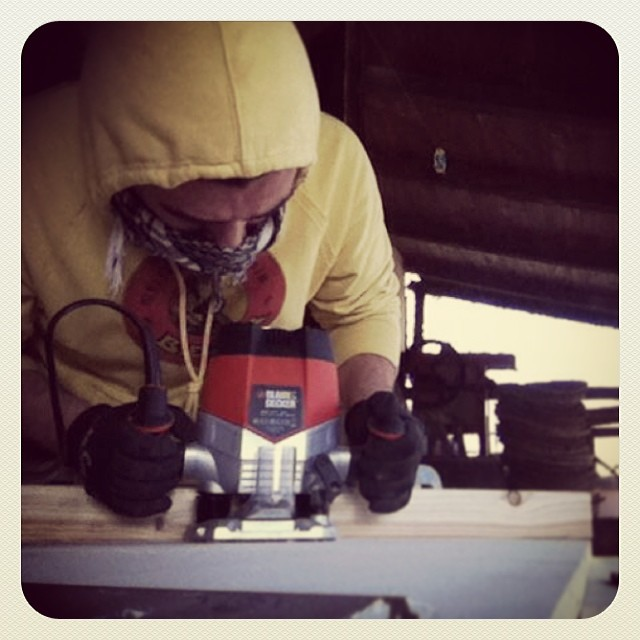
\includegraphics[width=.47\textwidth]{img/image2.jpg}
	\caption{Mappa della disposizione dei microfoni}
	\label{gs}
\end{figure}

\subsection*{Ruoli di ciascun punto di ripresa}
Ciascuno dei microfoni ha un ruolo preciso all'interno della ripresa dell'orchestra, in base a due parametri principali, ovvero:
A Coppia stereofonica della quale è parte
B Il suo posizionamento nello spazio: essendo i microfoni utilizzati identici tra loro (fatta eccezione per l'ORTF), il loro carattere dipende solo ed esclusivamente dal loro posizionamento. E' solo in base a questo che la sonorità dell'ambiente e della fonte sonora cambia nella ripresa.

\subsubsection{L'ORTF}
Il punto di ripresa principale è costituito da un ORTF, ovvero una coppia stereofonica semi spaziata con una distanza di 17cm circa tra le due capsule (circa la stessa distanza che intercorre tra le orecchie in un cranio umano) inclinate di 110° circa che permette di riprendere l'ambiente in maniera tridimensionale, fornendo informazioni relative alla profondità dell'ambiente acustico.
La caratteristica principale del modello ORTF sta nella sua naturalezza nel catturare l'ambiente: diversamente da una situazione in ambiente DAW, questa coppia semi-spaziata permette di catturare le fonti con i loro rispettivi ritardi, fornendo informazioni sulla reale provenienza del suono in base al ritardo che intercorre tra le due capsule microfoniche nel catturarla.
In questo caso, L'ORTF è stato posto di fronte all'orchestra in corrispondenza del pianoforte e del direttore d'orchestra, a fronte palco.

\subsubsection {I 10 Line Audio modello Omni1}
Anzitutto, a proposito dei microfoni omni-direzionali, c'è da precisare che questo tipo di microfono non ha una linearità nella direzionalità: si comportano diversamente a seconda delle frequenze che catturano. Certo non sono tutti uguali dunque questo andamento non lineare è più accentuato in alcuni microfoni e meno in altri, ma in linee generiche la tendenza è quella di limitare la sua direzionalità al crescere delle frequenze catturate stringendo la figura polare rendendola più simile a quella di un cardioide. Nella figura 2 è presente il diagramma polare e la risposta in frequenza del Line Audio - Omni1.

\begin{figure}[b]
	\begin{center}
		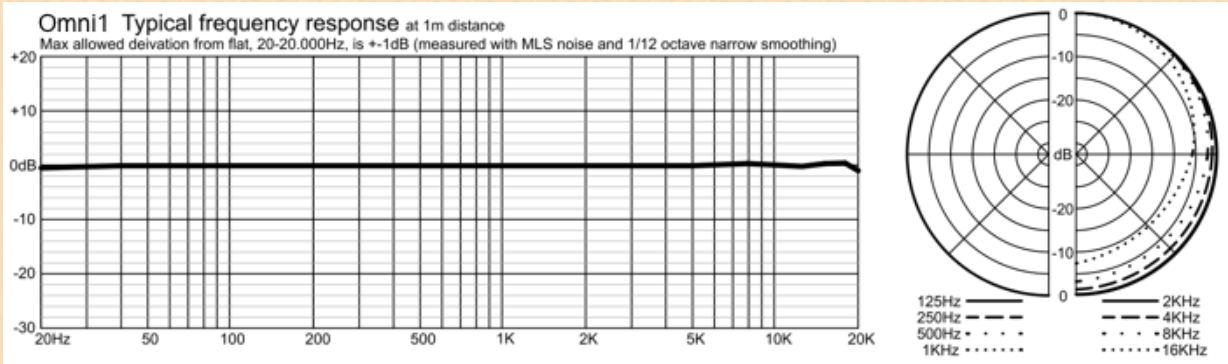
\includegraphics[width=.47\textwidth]{img/image1.png}
		\caption{\textbf{Caratteristiche del microfono di marca Line Audio modello Omni1}. Diagramma polare e risposta in frequenza.}
		\label{gr01}
	\end{center}
\end{figure}

I 10 microfoni sono stati così disposti:

Uno per i primi violini ed uno per le viole, posizionati specularmente nell'orchestra a distanza di 425cm l'uno dll'altro.

Tre per i fiati, dei quali uno centrale e due laterali, per allargarne l'immagine. Per questa sezione sono stati utilizzati tre microfoni per due motivi principali:
A La sezione è molto ampia(428cm)
B Per catturare anche i timpani, e in particolar modo il loro dettaglio, essendo storicamente utilizzati per dare sostegno ai fiati aggiungendo attacco e corpo al  suono.

Due in configurazione stereo AB L/R a distanza di 28cm l'uno dall'altro per il pianoforte per catturarne il dettaglio da vicino.

Uno come spot per i contrabbassi, posto a 309cm dal flankR. La sua utilità sta nel compensare il loro dettaglio che sicuramente manca al resto. C'è da precisare che questo punto di ripresa non potrebbe dare informazioni sulla profondità della sezione trattandosi di un microfono mono, così come non potrebbe riprenderne fedelmente le basse frequenze essendo un microfono di spot e quindi molto vicino alla sorgente, anche perchè le basse frequenze dei contrabbassi, così come degli altri strumenti (in particolar modo dei timpani), saranno già riprese fedelmente dai microfoni main, essendo questi molto distanti dalla sorgente.

Due utilizzati come Flanks, ovvero di sostegno all'ORTF a distanza speculare di 324cm per allargarne l'immagine. Il complesso Flanks + ORTF costituisce la ripresa MAIN dell'orchestra, ovvero quella generale, la quale non serve a catturare i singoli dettagli, quanto a dare un'immagine complessiva frontale del corpo dell'orchestra.


\section*{Gestione del materiale}
Premesso che:
A Al fine di realizzare un complesso sonoro unitario, il posizionamento dei microfoni è stato pensato per riprendere i dettagli di ogni sezione
B Il carattere timbrico di ogni singolo microfono dipende dalla sua posizione nello spazio,

Le modifiche spettrali e di fase applicate in fase di post produzione, sono anch'esse volte al raggiungimento di quest'obiettivo.
Dunque occorre organizzare le tracce affinchè ciascuna di esse abbia un ruolo preciso come componente del prodotto finale.

\subsection*{Sessione di registrazione}
Come interfaccia audio è stato utilizzato il mixer digitale di marca Allen e Heat, modello SQ5. I canali sono stati mappati sulla DAW Reaper. Dopo aver impostato i volumi allo stesso livello e acceso le Phantom power su tutti i canali, è stata avviata la registrazione.

\subsection*{Equalizzazione del materiale}
Terminata la registrazione, le tracce sono state disposte all'interno della DAW con un criterio di raggruppamento che organizza le registrazioni in diverse folder tracks: MAIN(ORTF, Flanks), FIATI(Fiati Left, Fiati Right, Fiati Center), VIOLINI/VIOLE(Secondi Violini, Viole).
Un'operazione importante è sicuramente filtrare le registrazioni di ogni singolo punto di ripresa al fine di far emergere il dettaglio della sezione in questione dallo spettro e, al contempo, tagliare le frequenze che compromettono questo approccio.
Ad esempio: Nelle registrazioni dei fiati è utile eliminare le basse frequenze, in quanto la loro utilità è catturare il dettaglio dei fiati nel loro range spettrale e il dettaglio delle membrane dei timpani, i quali servono a sostenere i fiati. Le basse frequenze dei timpani saranno già catturate dai punti di ripresa MAIN, trattandosi di microfoni lontani, dove la loro distanza dalla sorgente sonora permette a quest'ultima di svilupparsi per tutta la sua lunghezza d'onda.
Di conseguenza filtriamo la sezione dei fiati con un passa basso di terzo ordine a 200Hz, e la ripresa MAIN con un High Shelf a -3dB intorno ai 2500Hz per lasciare spazio alla ripresa dei fiati.
Lo stesso ragionamento va applicato ai contrabbassi, ad esempio.

\subsection*{Trattamento del materiale Mid/Side}
Perchè trattare il materiale delle registrazioni in Mid Side?
In questa configurazione, si può gestire l'ambiente come uno spazio trigonometrico, in quanto è possibile percepire la profondità di una fonte sonora nello spazio acustico nel quale suona, rimanendo fedeli al concetto di stereofonia.
Ma procediamo per steps.
Tutti gli spot utilizzati in fase di registrazione sono mono, dunque la prima cosa da fare è sicuramente metterli in correlazione con il punto di ripresa MAIN per poterci fare un'idea del posizionamento che  gli vogliamo dare nell'immagine stereo.
Procediamo con il routing Mid/Side creando una folder track che fungerà da matrice per ogni coppia separata. Quindi usiamo le seguenti formule per ottenere e poi miscelare Mid e Side separati

\begin{equation}
	Mid = Left(-3dB) + Right(-3dB)
	\label{eq:mid}
\end{equation}

\begin{equation}
	Side = Left(-3dB) - Right(-3dB)
	\label{eq:mid}
\end{equation}

Una volta create le folder M/S per ciascuna coppia, equalizziamo separatamente Mid e Side facendo in modo che i bassi dominino nel Mid e viceversa, per evitare cancellazioni di fase tra i due e per orientare le bande dello spettro nella nostra immagine stereo, nella quale avremo il corpo, la presenza e le basse frequenze al centro, e le informazioni stereofoniche (relative quindi all'ambiente nel quale suona l'orchestra) sul Side. Così facendo avremo una configurazione nella quale è possibile percepire al contempo presenza, corpo, dettagli e informazioni relative allo spazio acustico.


\vfill\null

\newpage % USE NEWPAGE TO FORCE COLUMNN INTERRUPTION
%-------------------------------------------------------------------------------
%-------------------------------------------------------------------------------

\begin{table}[htp]
\begin{tabular}{ll}
\textbf{Sommario} & \textbf{Page} \\
\hline
\textbf{Disposizione dei microfoni} & 1 \\
Ruoli di ciascun punto di ripresa & \\
L'ORTF & \\
I 10 Line Audio modello Omni1 & \\
\hline
\textbf{Gestione del materiale} & 2 \\
Sessione di registrazione & \\
Trattamento del materiale Mid/Side & \\

\end{tabular}
\end{table}

%--------------------------------------------
%----------------larghezza massima del codice

\vfill\null

\raggedright
%\bibliographystyle{unsrt}
%\printbibliography

\end{document}

%%%%%%%%%%%%%%%%%%%%%%%%%%%%%%%%%%%%%%%%%%%%%%%%%%%%%%%%%%%%%%%%%%%%%%%%%%%%%%%%
% 2020 GIUSEPPE SILVI ARTICLE TEMPLATE BASED ON
%%%%%%%%%%%%%%%%%%%%%%%%%%%%%%%%%%%%%%%%%%%%%%%%%%%%%%%%%%%%%%%%%%%%%%%%%%%%%%%%
% Journal Article
% LaTeX Template
% Version 1.4 (15/5/16)
% This template has been downloaded from:
% http://www.LaTeXTemplates.com
% Original author:
% Frits Wenneker (http://www.howtotex.com) with extensive modifications by
% Vel (vel@LaTeXTemplates.com)
% License:
% CC BY-NC-SA 3.0 (http://creativecommons.org/licenses/by-nc-sa/3.0/)
%%%%%%%%%%%%%%%%%%%%%%%%%%%%%%%%%%%%%%%%%%%%%%%%%%%%%%%%%%%%%%%%%%%%%%%%%%%%%%%%
